\documentclass[fleqn]{article}
\oddsidemargin 0.0in
\textwidth 6.0in
\thispagestyle{empty}
\usepackage{import}
\usepackage{amsmath}
\usepackage{graphicx}
\usepackage{flexisym}
\usepackage{calligra}
\usepackage{amssymb}
\usepackage{bigints} 
\usepackage[english]{babel}
\usepackage[utf8x]{inputenc}
\usepackage{float}
\usepackage[colorinlistoftodos]{todonotes}


\DeclareMathAlphabet{\mathcalligra}{T1}{calligra}{m}{n}
\DeclareFontShape{T1}{calligra}{m}{n}{<->s*[2.2]callig15}{}
\newcommand{\scriptr}{\mathcalligra{r}\,}
\newcommand{\boldscriptr}{\pmb{\mathcalligra{r}}\,}

\definecolor{hwColor}{HTML}{442020}

\begin{document}

  \begin{titlepage}

    \newcommand{\HRule}{\rule{\linewidth}{0.5mm}}

    \center

    \begin{center}
      
\includegraphics[height=11cm, width=11cm]{asu.png}
    \end{center}

    \vline

    \textsc{\LARGE Statistical/Thermal Physics}\\[1.5cm]

    \HRule \\[0.5cm]
    { \huge \bfseries Homework 12}\\[0.4cm] 
    \HRule \\[1.0cm]

    \textbf{Behnam Amiri}

    \bigbreak

    \textbf{Prof: Michael Treacy}

    \bigbreak

    \textbf{{\large \today}\\[2cm]}

    \vfill

  \end{titlepage}

  \begin{enumerate}
    \item \textbf{6.27} Use a computer to soum the exact rotational partition function (equation $6.30$) numerically, and 
    plot the result as a function of $kT/ \epsilon$. Keep enough terms in the sum to be confident that the series has converged.
    Show that the approximation in equation $6.31$ is a bit low, and estimate by how much. Explain the discrepancy by 
    referring to Figure $6.7$.

      \begin{center}
        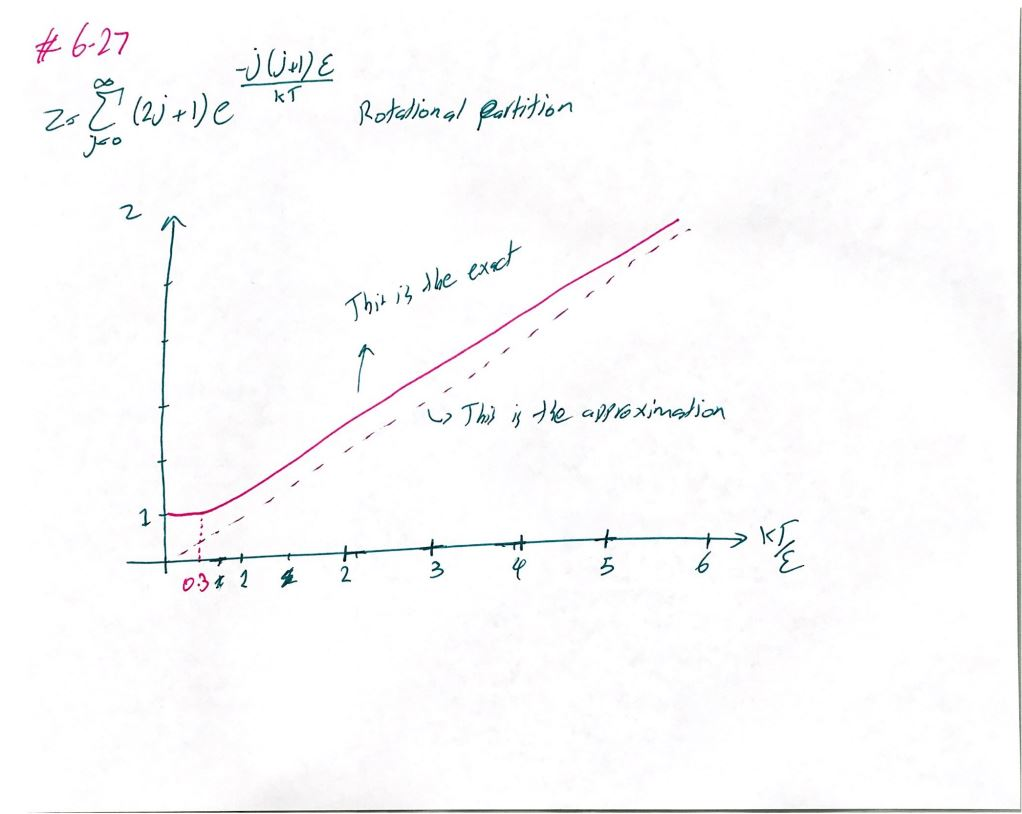
\includegraphics[height=16cm, width=16cm]{627.JPG}
      \end{center}

    \pagebreak

    \item \textbf{6.32} Consider a classical particle moving in a one-dimesional potential well $u(x)$....

      \begin{center}
        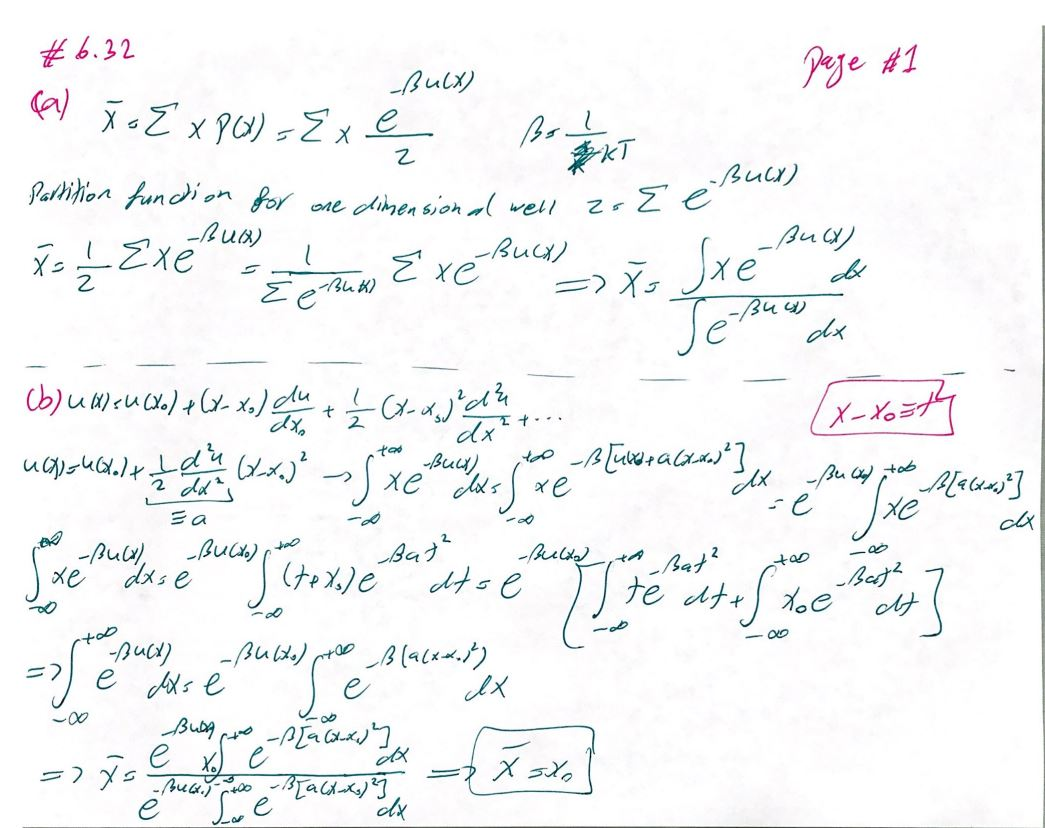
\includegraphics[height=16cm, width=16cm]{632A.JPG}
      \end{center}
      \pagebreak
      \begin{center}
        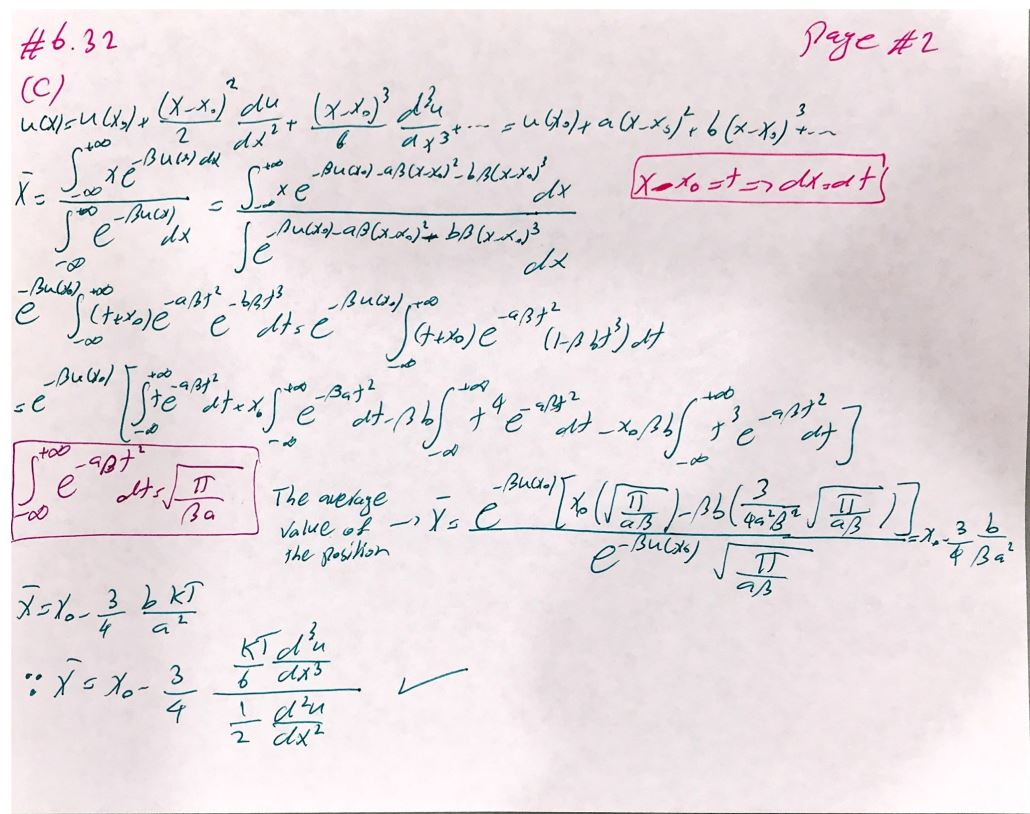
\includegraphics[height=15cm, width=16cm]{632B.JPG}
      \end{center}
      \pagebreak
      \begin{center}
        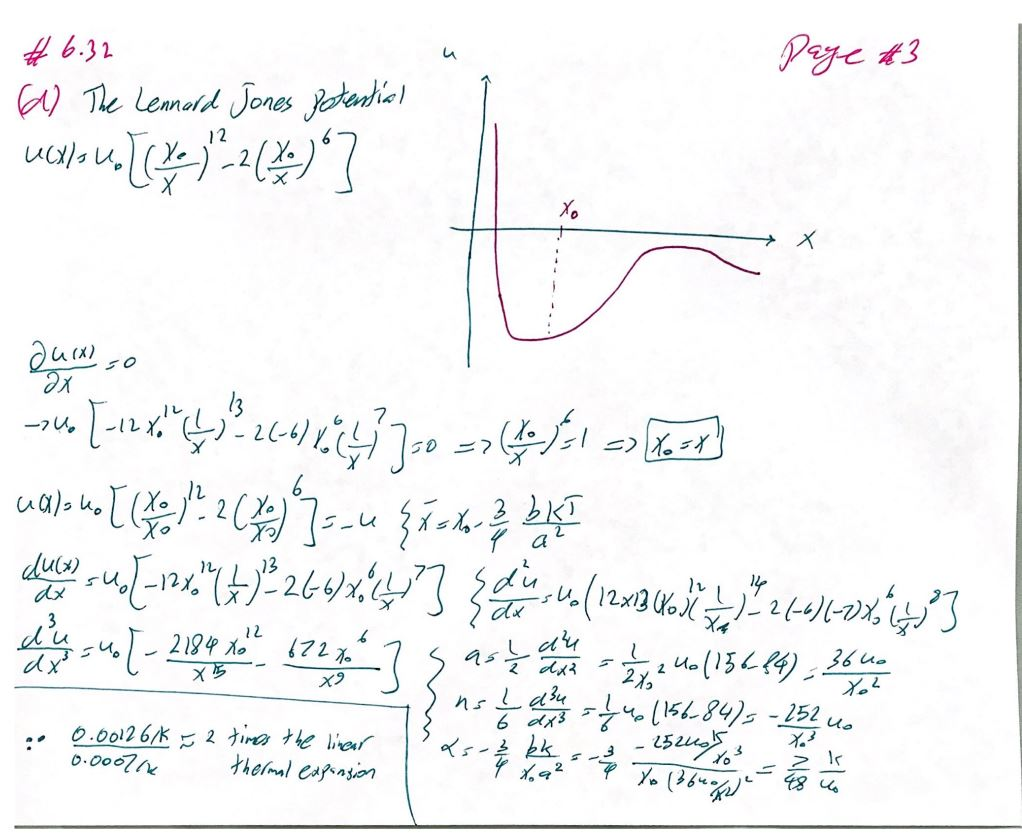
\includegraphics[height=15cm, width=16cm]{632C.JPG}
      \end{center}

    \pagebreak

    \item \textbf{6.34} Carefully plot Maxwell speed distribution for nitrogen molecules at $T=300 ~ K$ and at 
    $T=600 ~ K$. Plot both graphs on the same axes, and label the axes with numbers.

      \begin{center}
        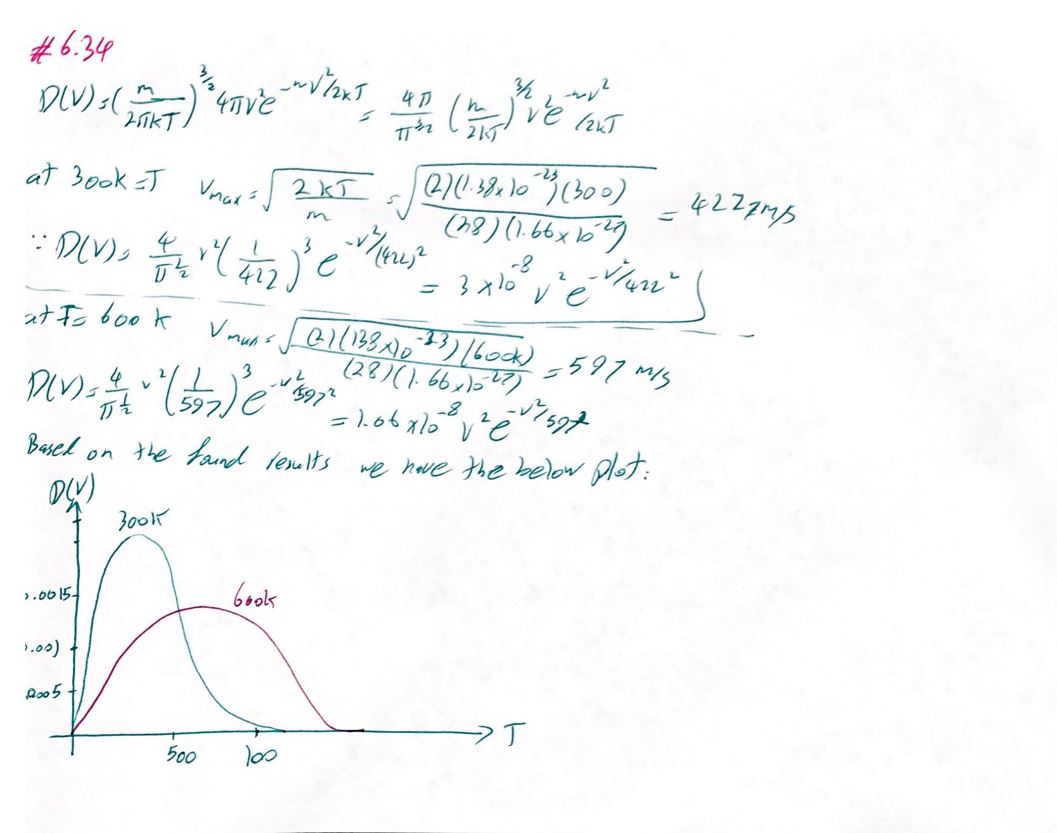
\includegraphics[height=15cm, width=18cm]{634.JPG}
      \end{center}

    \pagebreak

    \item \textbf{6.39} A particle near earth's surface traveling faster than about $11 km/s$ has enough...

      \begin{center}
        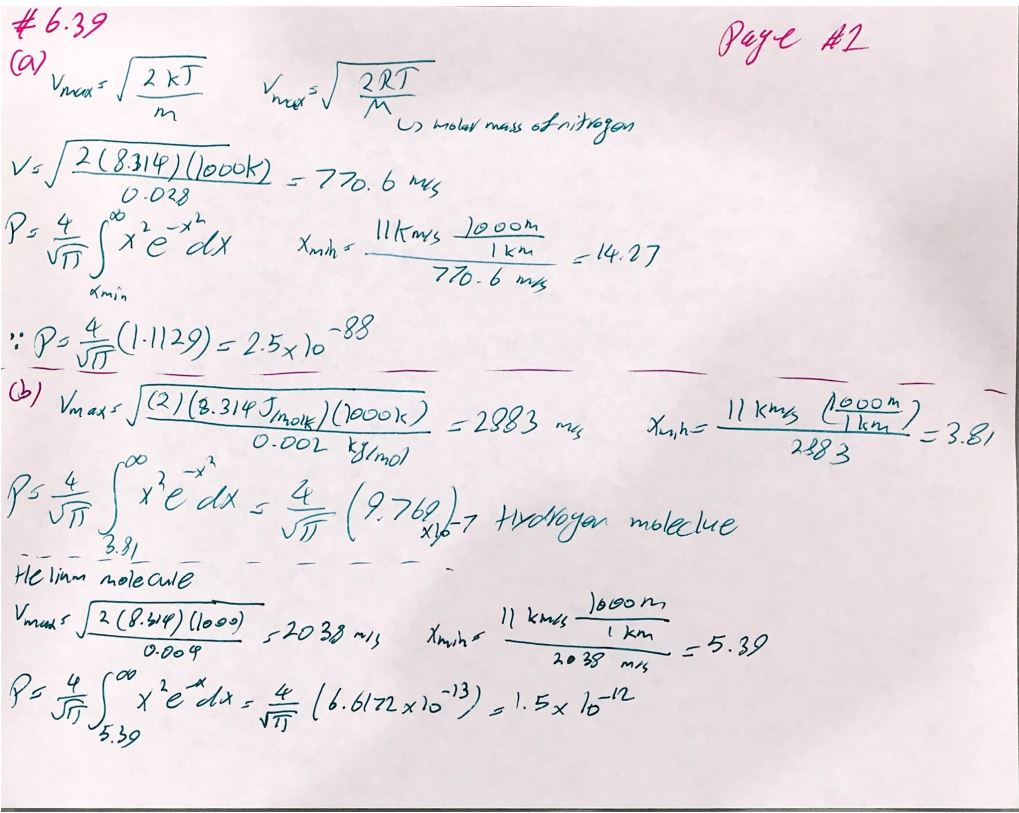
\includegraphics[height=15cm, width=16cm]{639A.JPG}
      \end{center}
      \pagebreak
      \begin{center}
        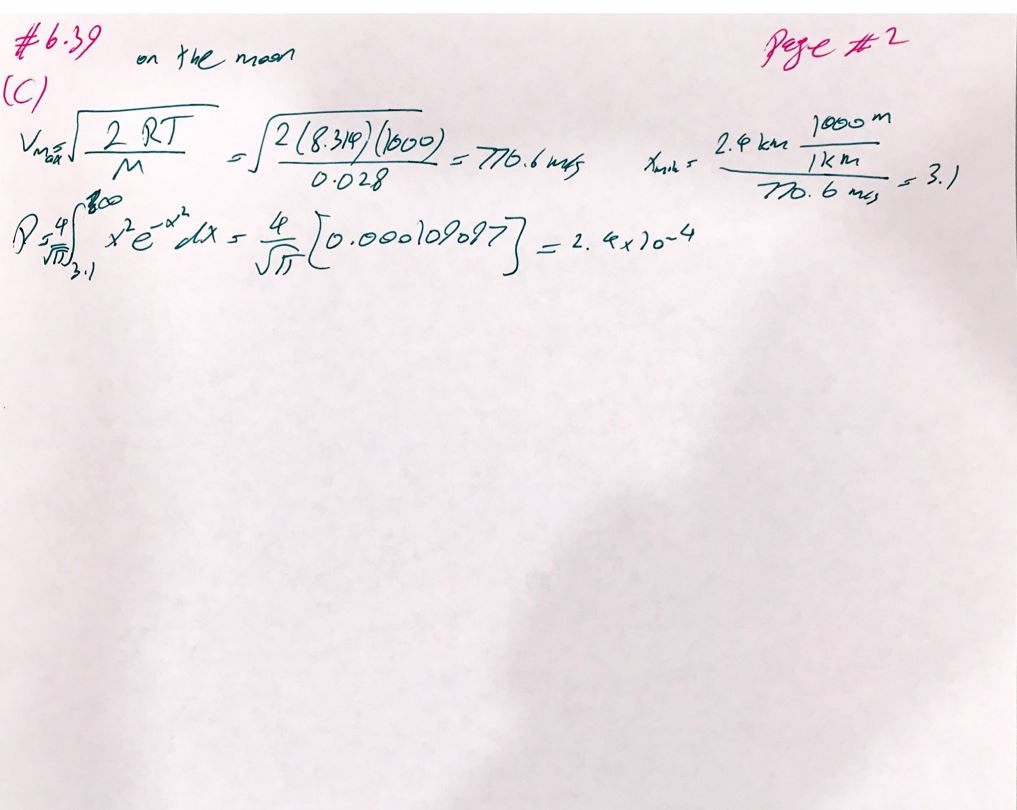
\includegraphics[height=15cm, width=16cm]{639B.JPG}
      \end{center}

    \pagebreak

    \item \textbf{6.43} Some advanced textbooks define entropy...

      \begin{center}
        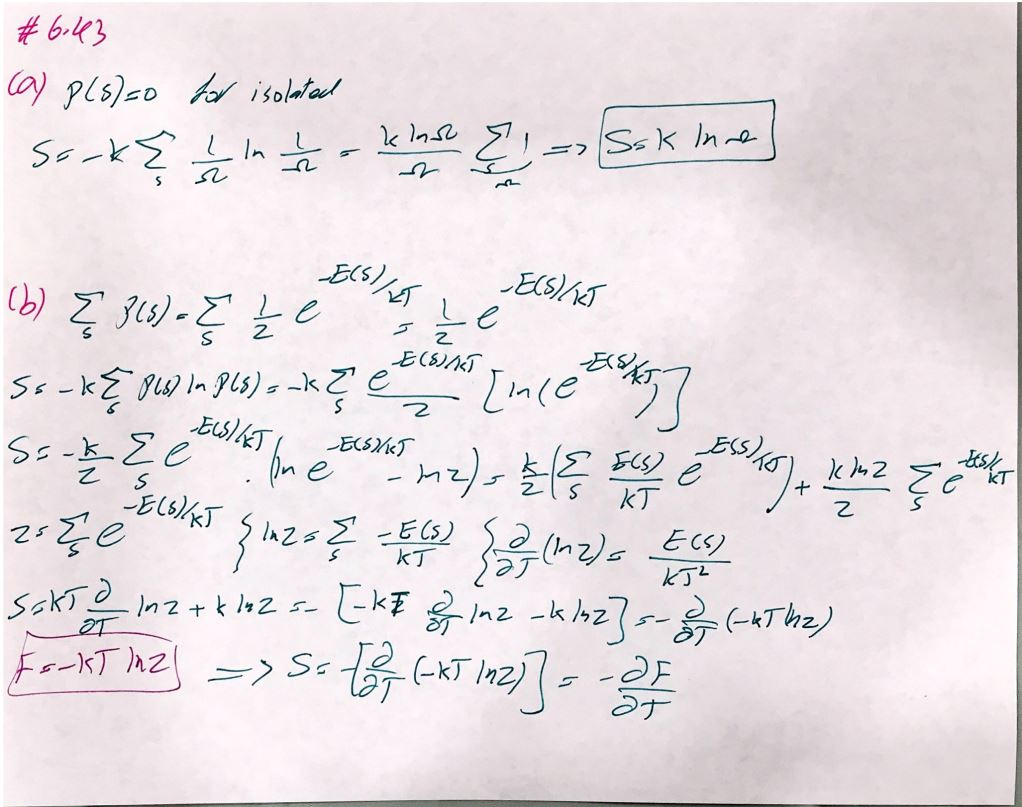
\includegraphics[height=15cm, width=16cm]{643.JPG}
      \end{center}

    \pagebreak

    \item \textbf{6.48} For a diatomic gas near room temperature, the internal partition function is simply...  

      \begin{center}
        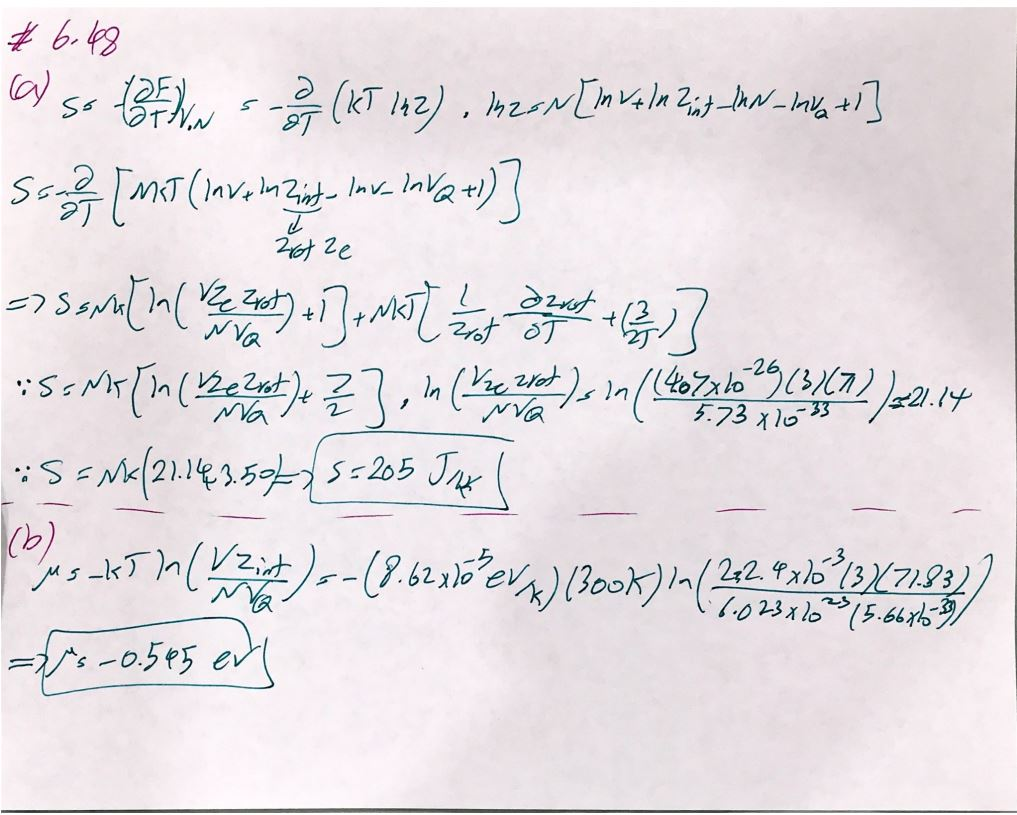
\includegraphics[height=15cm, width=16cm]{648.JPG}
      \end{center}

    \pagebreak

  \end{enumerate}

\end{document}
